\section{Modularity}
\label{sec:modularity}
\fxfatal{Modularity}

\subsection{Definition}

\begin{quote}
Large software systems are inherently more complex to develop and maintain than smaller systems. Modularity involves breaking a large system into separate physical entities that ultimately makes the system easier to understand. By understanding the behaviors contained within a module and the dependencies that exist between modules, it’s easier to identify and assess the ramification of change.

\hfill \textbf{Java Application Architecture}

\hfill \citeauthor{Knoernschild:2012} \cite{Knoernschild:2012}
\end{quote}

\begin{quote}
The term modularity is widely used in studies of technological and organizational systems. Product systems are deemed “modular”, for example, when they can be decomposed into a number of components that may be mixed and matched in a variety of configurations. The components are able to connect, interact, or exchange resources (such as energy or data) in some way, by adhering to a standardized interface. Unlike a tightly integrated product whereby each component is designed to work specifically (and often exclusively) with other particular components in a tightly coupled system, modular products are systems of components that are “loosely coupled.

\hfill \textbf{Modularity}

\hfill \citeauthor{Wikipedia:Modularity:2012} \cite{Wikipedia:Modularity:2012}

\end{quote}

\newpage
\subsection{OSGi}
The \gls{OSGi} technology is a set of specifications that define a dynamic component system for Java. These specifications enable a development model where applications are dynamically composed of many different reusable components. The \gls{OSGi} specifications enable components to hide their implementations from other components while communicating through services, which are objects that are specifically shared between components. This surprisingly simple model has far reaching effects for almost any aspect of the software development process \cite{OSGi}. In OSGi parlance, a module is known as a bundle. OSGi provides a framework for managing bundles that are packaged as regular Java JAR files with an accompanying manifest. The manifest contains important metadata that describes the bundles and its dependencies to the OSGi framework \cite{Knoernschild:2012}. Figure \ref{fig:layering-osgi} shows the layered model architecture of the \gls{OSGi} service platform.

\begin{figure}[H]
\centering
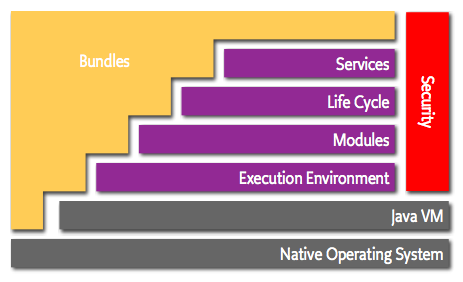
\includegraphics[width=\textwidth]{layering-osgi.png}
\caption{\gls{OSGi} layered model \cite{OSGi}}
\label{fig:layering-osgi}
\end{figure}

\newpage
In summary, the \gls{OSGi} service platform offers the following features \cite{Knoernschild:2012}:

\begin{enumerate}
	\item \textbf{Modularity}: \\
	Enables and enforces a modular approach to architecture on the Java platform.
	\item \textbf{Versioning}: \\
	Supports multiple versions of the same software module deployed within the same Java Virtual Machine (JVM) instance.
	\item \textbf{Hot deployments}: \\
	Permits modules to be deployed and updated within a running system without restarting the application or the JVM.
	\item \textbf{Encapsulation}: \\
	Allows modules to hide their implementation details from consuming modules.
	\item \textbf{Service orientation}: \\
	Encourages service-oriented design principles in a more granular level within the JVM. To accomplish this, OSGi uses $\mu$Services.
	\item \textbf{Dependency management}: \\
	Requires explicit declaration of dependencies between modules.
\end{enumerate}